\documentclass[10pt]{standalone}

\usepackage{pgf,tikz}
\usepackage{mathrsfs}
\usetikzlibrary{arrows}
\pagestyle{empty}
\newcommand{\conj}[2][3]{{}\mkern#1mu\overline{\mkern-#1mu#2}}
\let\misura\conj
\begin{document}

	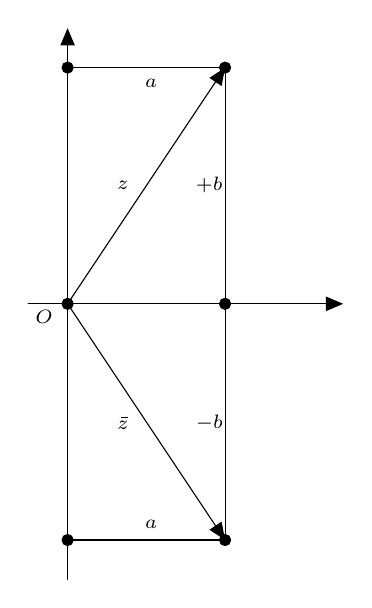
\begin{tikzpicture}[line cap=round,line join=round,>=triangle 45,x=1.0cm,y=1.0cm]
	\draw[->] (-0.5,0.) -- (3.5,0.);
	
	\draw[->] (0.,-3.5) -- (0.,3.5);
	
	\clip(-0.5,-3.5) rectangle (3.5,3.5);
	\draw [->] (0.,0.) -- (2.,3.);
	\draw [->] (0.,0.) -- (2.,-3.);
	\draw  (2.,3.)-- (2.,-3.);
	\draw  (2.,3.)-- (0.,3.);
	\draw  (2.,-3.)-- (0.,-3.);
	\begin{scriptsize}
	\draw [fill=black] (0.,0.) circle (2.0pt);
	\draw (-0.3,-0.17) node {$O$};
	\draw [fill=black] (2.,3.) circle (2.0pt);
	\draw (0.7,1.51) node {$z$};
	\draw [fill=black] (2.,-3.) circle (2.0pt);
	\draw (0.7,-1.51) node {$\conj{z}$};	
	\draw (1.8,1.51) node {$+b$};
	\draw (1.8,-1.51) node {$-b$};
	\draw [fill=black] (0.,3.) circle (2.0pt);
	\draw (1.06,2.8) node {$a$};
	\draw [fill=black] (0.,-3.) circle (2.0pt);
	\draw (1.06,-2.8) node {$a$};
	\draw [fill=black] (2.,0.) circle (2.0pt);
	\end{scriptsize}
	\end{tikzpicture}
\end{document}